\documentclass[a4paper,10pt]{article}
\usepackage[utf8x]{inputenc}

% Pacotes 
\usepackage[brazil]{babel} 
%\usepackage[latin1]{inputenc}
\usepackage{amsfonts}
\usepackage{amssymb} 
\usepackage{indentfirst} 	% indentacao do primeiro paragrafo
\usepackage{cite}  		% modo de citacao legal


%\usepackage{makeidx} 		% índice remissivo
\usepackage[nottoc]{tocbibind}  % acrescentamos a bibliografia/indice/conteudo no Table of Contents
\usepackage{setspace}

% By David
\usepackage[dvips]{graphicx} 	% ou usa [dvips]{graphicx} ou {pdfpages}
%\usepackage{pdfpages}		% permite o use de ``includepdf''
\usepackage{amsthm}
\usepackage{acronym} 
%\usepackage[portugues,ruled,vlined,linesnumbered]{algorithm2e/algorithm2e}
\usepackage{supertabular}
%\usepackage[margin=3cm,noheadfoot]{geometry}


%opening
\title{Tabuleiro Eletrônico com Arduino}
\author{}
\date{}

\begin{document}

\maketitle

\begin{abstract}
Os jogos de tabuleiro fazem parte da cultura desde tempos imemoriais. Normalmente são jogados por ao menos duas pessoas, mas existem alguns que admitem uma quantidade muito maior de jogadores. Entretanto, nas duas últimas décadas este tipo de jogo perdeu muito espaço devido aos jogos eletrônicos. \\ 

Para cada um dos diferentes tipos de jogos de tabuleiro desde guerra, estratégia, {\it RPG}, eliminatórios, de festa ou mesmo infantis, um tipo de tabuleiro distinto é preciso. Dentro de uma mesma categoria, uma quantidade significativamenete grande de diferentes jogos em diferentes versões são encontrados, sendo que cada uma possui um tabuleiro, quase sempre, distinto dos demais. Apesar deste imenso conjunto de tabuleiros distintos, torna-se cansativo jogar determinado jogo sempre em mesmo tabuleiro. \\

A proposta deste projeto é construir um tabuleiro eletrônico, a qual possa, por meio de um sistema computacional, ``contruir'' instantaneamente um tabuleiro a ser utilizado em determinado jogo. \\

%\cleardoublepage
\noindent \textbf{Palavras-chave:} tabuleiro eletrônico, mesa digital, jogos.
\end{abstract}


% OBSERVAÇÂO: Durante a construção da mesa, isto é, enquanto este texto for uma PROPOSTA, o tempo verbal sera no futuro. Exemplo: ''a mesa terá...''
% Após a finalização do projeto o tempo verbal deverá ser modificado para o presente. Exemplo: ''a mesa tem...''

\section{Introdução}

A estrutura principal da mesa será composta por um conjunto de celulas hexagonais e retangulares, que ficarão sob um tampo de vidro fumê. 
Cada uma células hexagonais será composta por dois LEDs RGB separado por uma divisoria que cortará ao meio a célula. 
A célula hexagonal será construida com acrílico com espessura de 5mm. Sendo que abaixo de cada uma das facetas de acrílico do hexagono terá um LED monocro\-mático.
%Desta maneira ao ser ligado os LEDs sob...
Cada uma das células retangulares será composta por um unico LED monocromático. \\

Cada uma dos LEDs (RGBs ou monocromáticos) poderá ser controlado individualmente.

\section{Descrição}

A central de controle da mesa sera composta por um Arduino com conexão WiFi (um shield ou um BlackWidow) e um conjunto de Rainbowduino. \\

\begin{center}
\begin{figure}[h!]
	\center
	\includegraphics[angle=0, scale=0.40]{./img/layout-v02.ps}
	\label{figura_layout}
	\caption{Projeção da mesa eletrônica visto de cima.}
\end{figure}
\end{center}

\subsection{Estrutura}

Cada exagono que compõe a estrutura central da mesa terá dois LEDs RGB de 5mm. A di, separados por uma divisoria 

\begin{center}
\begin{figure}[h!]
	\center
	\includegraphics[angle=0, scale=0.25]{./img/prototipo-projeto-mesa-v02-b.ps}
	\label{figura_prototipo}
	\caption{Visualização dos hexagonos que compõe a estrutura.}
\end{figure}
\end{center}

\begin{center}
\begin{figure}[h!]
	\center
	\includegraphics[angle=0, scale=0.40]{./img/projeto-v02.ps}
	\label{figura_projeto}
	\caption{Projeção da mesa eletrônica incluindo a visualização interna dos componentes estruturais.}
\end{figure}
\end{center}


\subsection{Hardware}

\subsubsection{Componentes}

\subsection{Software}



\section{Cronograma}

\section{Modulos Adicionais}

\subsection{LEDs de Alto Brilho}

\subsection{Sensores Infravermelho}

\subsection{Entrada e Saída de Audio}

\section{Projetos Relacionados}

\subsection{Microsoft Surface}
\subsection{Philips Entertaible}
\subsection{DiamondTouch}


\section{Referências}

\begin{verbatim}
Wikipédia
 http://pt.wikipedia.org/wiki/Jogo_de_tabuleiro
 http://pt.wikipedia.org/wiki/Lista_de_jogos_de_tabuleiro 
\end{verbatim}

\end{document}
